\section{Long Short Term Memories (LSTM)}
\subsection{Định nghĩa}

Long Short Term Memories (LSTM) là một biến thể của mô hình Recurrent neural network  RNN (hình 1) với cấu trúc mạng được tổng hợp từ nhiều đơn vị Long short-term memory. Một đơn vị LSTM gồm có nhân (cell), một cổng vào (input gate), một cổng ra (output gate) và một cổng quên (forget gate). Sơ đồ minh hoạt cho một đơn vị LSTM được thể hiện ở hình 1.2.

\begin{figure}[!htp]
	\centering
	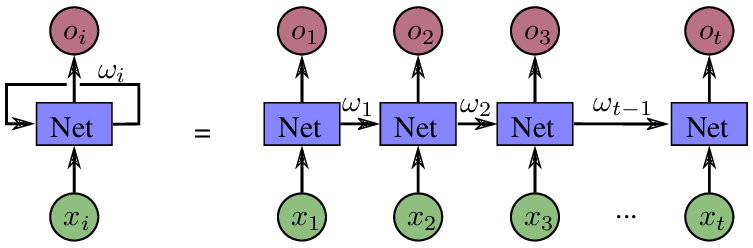
\includegraphics[scale=.5]{hinhanh/RNN.png}
	\caption{Một dạng mô hình RNN}
\end{figure} 


\begin{figure}[!htp]
	\centering
	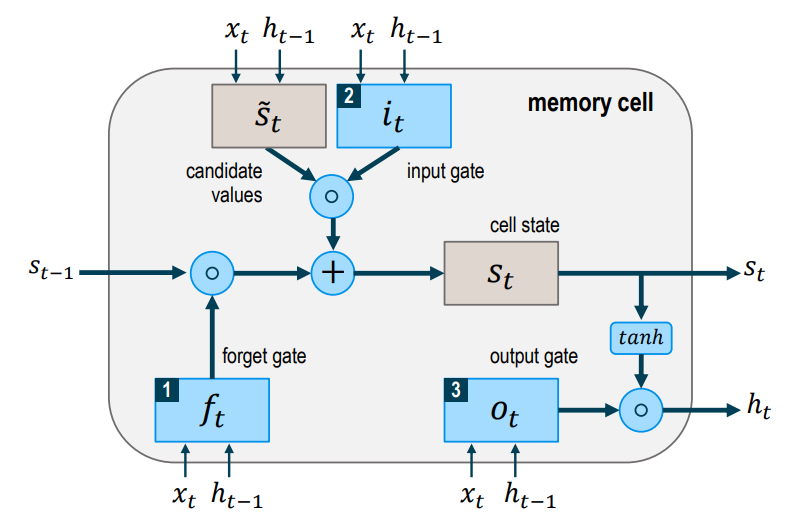
\includegraphics[scale=.7]{hinhanh/LSTM.png}
	\caption{Cấu trúc của một nhân LSTM}
\end{figure} 

Vì có khả năng nhớ nên LSTM rất phù hợp với bài toán phân loại và dự báo dựa trên dữ liệu dạng chuỗi thời gian. Hơn nữa LSTM còn có đặt trưng loại bỏ được hiện tượng triệt tiêu (vanishing) và bùng nổ (exploding) gradient.

\subsection{Cơ chế hoạt động}

Như đã giới thiệu ở trên, mỗi đơn vị LSTM có nhiều cổng khác nhau, tương ứng với các chức năng khác nhau:

\begin{itemize}
	\item \textbf{Forget gate:} Cổng này quyết định xem thông tin nào trong bộ nhớ hiện tại được giữ và thông tin nào bị bỏ lại. Thông tin đầu vào được cho vào hàm signoid. Đầu ra của hàm này đóng vai trò là mask để lọc thông tin từ trạng thái nhân.
	\item \textbf{Input gate:} Cổng này dùng để cập nhật bộ nhớ với các thông tin mới. Ở đây có xuất hiện 2 hàm sigmoid và hàm tanh. Tác dụng của chúng cũng như trên. Output từ hàm sigmoid sẽ có tác dụng lọc thông tin đã qua xử lý từ output hàm tanh.
	\item \textbf{Output gate:} cổng này quyết định output của từ hiện tại là gì. Nó được lấy thông tin từ 2 nguồn: trạng thái nhân và input hiện tại. Trạng thái cell sau khi chỉnh sửa sẽ đi qua hàm tanh và input hiện tại thì được đi qua hàm sigmoid. Từ đây ta kết hợp 2 kết quả trên để có được kết quả đầu ra. Chú ý rằng cả kết quả đầu ra và cả trạng thái cell đều được đưa vào bước tiếp theo.
\end{itemize}

\subsection*{Các biến số}
Trước khi đi vào chi tiết quá trình hoạt động của LSTM, ta cần hiểu ý nghĩa của các giá trị dưới đây:

\begin{itemize}
	\item $ x_t $ là vector đầu vào tại bước thời gian $ t $
	\item $ {W_{f,x}},{W_{f,h}},{W_{\mathop s\limits^ \sim  ,x}},{W_{\mathop s\limits^ \sim  ,h}},{W_{i,x}},{W_{i,h}},{W_{o,x}},{W_{o,h}} $ là các ma trận trọng số trong mỗi tế bào.
	\item $ {b_f},{b_{\mathop s\limits^ \sim  }},{b_i},{b_o} $ là các véc tơ bias.
	\item $ {f_t},{i_t},{o_t} $ là các hàm kích hoạt tại forget gate, input gate và output gate.
	\item $ {s_t},\mathop s\limits^ \sim $ là véc tơ trạng thái của nhân và giá trị đề cử (candidate value).
	\item $ h_t $ là tham số đầu vào của mỗi tế bào LSTM.
\end{itemize}

\subsection*{Forward}

Quá trình lan truyền xuôi (forward) của mạng LSTM được thực hiện như sau:
\begin{enumerate}
	\item Đầu tiên, một giá trị $ h_{t-1} $ ngẫu nhiên (hoặc được đặt sẵn) được tạo ra và làm tham số đầu vào cho nhân LSTM đầu tiên.
	\item Kế đến, nhân LSTM sẽ quyết định thông tin nào cần loại bỏ trong $ s_{t-1} $ thông qua hàm $ f_t $ dựa trên ba giá trị $ x_t $, $ h_{t-1} $ và bias $ b_f $ của $ f_t $. 
	\begin{center}
		$ {f_t} = \sigma \left( {{W_{f,x}}{x_t} + {W_{f,h}}{h_{t - 1}} + {b_f}} \right) $
		
		$
		i_t = \tanh ( W_{i,x}x_t + W_{i,h}h_{t - 1} + b_i)
		$
	\end{center}
	\item Sau đó, nhân LSTM sẽ quyết định thông tin nào sẽ được thêm vào $ s_t $ thông qua phép toán:
	\begin{equation}
	\mathop {{s_t}}\limits^ \sim   = \tanh \left( {{W_{\mathop s\limits^ \sim  ,x}}{x_t} + {W_{\mathop s\limits^ \sim  ,h}}{h_{t - 1}} + {b_{\mathop s\limits^ \sim  }}} \right)
	\end{equation}
	\item Tiếp theo, giá trị $ s_t $ sẽ được tính toán với phép nhân Hadamard theo từng phần tử $\circ$ (Hadamard prodcut).
	\begin{equation}
	{s_t} = {f_t} \circ {s_{t - 1}} + {i_t} \circ \mathop {{s_t}}\limits^ \sim
	\end{equation}
	\item Ở bước cuối cùng của một nhân, giá trị đầu ra $ h_t $ của nhân hiện tại và là đầu vào của nhân kế đó được tính bằng:
	\begin{equation}
	{h_t} = {o_t} \circ \tanh \left( {{s_t}} \right)
	\end{equation}
	Trong đó:
	\begin{equation}
	{o_t} = \sigma \left( {{W_{o,x}}{x_t} + {W_{o,h}}{h_{t - 1}} + {b_o}} \right)
	\end{equation}
	\item Quá trình 1-5 sẽ được thực hiện tuần tự lặp đi lặp lại cho đến nhân LSTM cuối cùng.
\end{enumerate}
